\begin{question*}
  We have $n$ data points $(x_{1}, y_{1}), \ldots, (x_{2}, y_{2})$. Find $y(x)$ which minimizes the sum of squares.
\end{question*}

How do we represent this as an integral of a differentiable Lagrangian?

Under the conventional least-squares criterion, the ``action'' is
\begin{align*}
  A[y] = \sum_{i=1}^{n} \(y(x_{i}) - y_{i}\)^{2}.
\end{align*}
We need to represent this as
\begin{align*}
  A[y] = \int_{y} \Lag(y, y', x),
\end{align*}
or
\begin{align*}
  A[y] = \int_{x_1}^{x_n} \Lag\(y(x), y'(x), x\) \dx.
\end{align*}
Let $p(x, y)$ be the penalty associated with point $(x, y)$ in a candidate curve.

I think we need to ``integrate along the curve''. I.e. what we are minimizing should be the total exposure to
this penalty function as we move along the curve in 2D.
\begin{align*}
  A[y]
  &= \int_y p(x, y) \\
  &= \int_{x_a}^{x_b} p(x, y) \sqrt{(\dx)^2 + (y'(x)\dx)^2} \\
  &= \int_{x_a}^{x_b} p(x, y) \sqrt{1 + (y'(x))^2} \dx
\end{align*}

\subsubsection*{Lagrangian I}

One choice of penalty function would be the sum of squared distances to all data points:
\begin{align*}
  p(x, y) = \sum_i (x - x_i)^2 + (y - y_i)^2.
\end{align*}
With this penalty function, the action to be minimized is
\begin{align*}
  A[y]
  &= \int_{x_1}^{x_n} \Lag\(y, y', x\) \dx \\
  &= \int_{x_a}^{x_b} \sqrt{1 + y'^2} \sum_i \((x - x_i)^2 + \(y - y_i\)^2\) \dx.
\end{align*}
The partial derivatives are
\begin{align*}
  \pdLdy  &= 2\sqrt{1 + y'^2} \sum_i \(y - y_i\) \\
  \pdLdyp &= \frac{y'}{\sqrt{1 + y'^2}}  \sum_i \((x - x_i)^2 + \(y - y_i\)^2\).
\end{align*}
Note that, via the quotient rule $\(\frac{f}{g}\)' = \frac{gf' - fg'}{g^2}$, we have
\begin{align*}
  \ddx \frac{y'}{\sqrt{1 + y'^2}}
  &= \frac{y''\sqrt{1 + y'^2} + y'\frac{1}{2}\frac{1}{\sqrt{1 + y'^2}}2y'y''}{1 + y'^2} \\
  &= \frac{y''}{\sqrt{1 + y'^2}} + \frac{y'^2y''}{(1 + y'^2)^{3/2}}.
\end{align*}
\begin{mdframed}
[Check]
\begin{minted}{wolfram} :results latex
D[y'[x]/Sqrt[1 + y'[x]^2], x]
\end{minted}

\begin{align*}
\frac{y''(x)}{\sqrt{y'(x)^2+1}}-\frac{y'(x)^2 y''(x)}{\left(y'(x)^2+1\right)^{3/2}}
\end{align*}
\begin{align*}
\frac{y''(x)}{\sqrt{y'(x)^2+1}}-\frac{y'(x)^2 y''(x)}{\left(y'(x)^2+1\right)^{3/2}}
\end{align*}
\end{mdframed}

Hence
\begin{align*}
  \ddx\pdLdyp
  &= \(\ddx \frac{y'}{\sqrt{1 + y'^2}}\)  \sum_i \((x - x_i)^2 + \(y - y_i\)^2\) + \frac{2y'}{\sqrt{1 + y'^2}}  \sum_i (x - x_i) \\
\end{align*}
And so the Lagrange equations are
\begin{align*}
  \ddx \pdLdyp - \pdLdy &= 0 \\
  \(\ddx \frac{y'}{\sqrt{1 + y'^2}}\)  \sum_i \((x - x_i)^2 + \(y - y_i\)^2\) + \frac{2y'}{\sqrt{1 + y'^2}}  \sum_i (x - x_i) - 2\sqrt{1 + y'^2} \sum_i \(y - y_i\) &= 0 \\
  \(\ddx \frac{y'}{\sqrt{1 + y'^2}}\) \sqrt{1 + y'^2} \sum_i \((x - x_i)^2 + \(y - y_i\)^2\) + 2y'  \sum_i (x - x_i) - 2(1 + y'^2) \sum_i \(y - y_i\) &= 0 \\
\end{align*}


\subsection*{Lagrangian II}

  Let's try a different Lagrangian: consider a point $(x, y)$ on the candidate curve, and consider data
  point $(x_i, y_i)$. If $x_i$ is close to $x$ but $y_i$ is far from $y$, then the Lagrangian should penalize
  the candidate curve. So define
  \begin{align*}
    p(x, y) = \sum_i \frac{(y - y_i)^2}{1 + (x - x_i)^2}.
  \end{align*}
With this penalty function, the action to be minimized is
\begin{align*}
  A[y]
  &= \int_{x_1}^{x_n} \Lag\(y, y', x\) \dx \\
  &= \int_{x_a}^{x_b} \sqrt{1 + y'^2} \sum_i \frac{(y - y_i)^2}{1 + (x - x_i)^2} \dx.
\end{align*}


The partial derivatives are
\begin{align*}
  \pdLdy &= 2\sqrt{1 + y'^2} \sum_i \frac{y - y_i}{1 + (x - x_i)^2} \\
  \pdLdyp &= \frac{y'}{\sqrt{1 + y'^2}}  \sum_i \frac{(y - y_i)^2}{1 + (x - x_i)^2},
\end{align*}
hence
\begin{align*}
  \ddx \pdLdyp &=
  \(\ddx \frac{y'}{\sqrt{1 + y'^2}}\) \sum_i \frac{(y - y_i)^2}{1 + (x - x_i)^2} -
  2\frac{y'}{\sqrt{1 + y'^2}} \sum_i \frac{(x - x_i)(y - y_i)^2}{\(1 + (x - x_i)^2\)^2}
\end{align*}
and Lagrange equations
\begin{align*}
  \(\ddx \frac{y'}{\sqrt{1 + y'^2}}\) \sum_i \frac{(y - y_i)^2}{1 + (x - x_i)^2} -
  2\frac{y'}{\sqrt{1 + y'^2}} \sum_i \frac{(x - x_i)(y - y_i)^2}{\(1 + (x - x_i)^2\)^2}
  - 2\sqrt{1 + y'^2} \sum_i \frac{y - y_i}{1 + (x - x_i)^2} &= 0 \\
  \(\ddx \frac{y'}{\sqrt{1 + y'^2}}\) \sum_i (y - y_i)^2 -
  2\frac{y'}{\sqrt{1 + y'^2}} \sum_i \frac{(x - x_i)(y - y_i)^2}{1 + (x - x_i)^2}
  - 2\sqrt{1 + y'^2} \sum_i (y - y_i) &= 0.
\end{align*}

\subsection*{Mathematica}

We want to obtain and solve the Lagrange equations  for various choices of penalty function.

First, let's check we know how to differentiate an expression w.r.t. $x$, $y$, and $y'$:

\begin{minted}{wolfram} :results latex
f = Sqrt[1 + (y'[x])^2];
{D[f, x], D[f, y[x]], D[f, y'[x]]}
\end{minted}

\begin{align*}
\left\{\frac{y'(x) y''(x)}{\sqrt{y'(x)^2+1}},0,\frac{y'(x)}{\sqrt{y'(x)^2+1}}\right\}
\end{align*}
\begin{align*}
\left\{\frac{y'(x) y''(x)}{\sqrt{y'(x)^2+1}},0,\frac{y'(x)}{\sqrt{y'(x)^2+1}}\right\}
\end{align*}

Compute the partial derivatives of the Lagrangian:

% \begin{minted}{wolfram} :results latex
% xobs = {-2, -1, 0, 1, 2};
% yobs = {4, 1, 0, 1, 4};
% n = Length[xobs]
% pen = Sum[(x - xobs[[i]])^2 + (y[x] - yobs[[i]])^2, {i, n}]; (* penalty function *)
% lag = pen Sqrt[1 + (y'[x])^2]; (* Lagrangian *)
% {D[lag, y[x]], D[lag, y'[x]]}
% \end{minted}

% \begin{align*}
% \left\{\sqrt{y'(x)^2+1} \left(\sum _i^n 2 (y(x)-\text{yobs}[[i]])\right),\frac{y'(x) \left(\sum _i^n \left((x-\text{xobs}[[i]])^2+(y(x)-\text{yobs}[[i]])^2\right)\right)}{\sqrt{y'(x)^2+1}}\right\}
% \end{align*}




% Now, $\ddx \pdLdyp$ is

% \begin{minted}{wolfram} :results latex
% p = (x - x1)^2 + (y[x] - y1)^2; (* penalty function *)
% lag = p Sqrt[1 + (y'[x])^2]; (* Lagrangian *)
% D[ D[lag, y'[x]], x]
% \end{minted}

% \begin{align*}
% \frac{y'(x) \left(2 (x-\text{x1})+2 (y(x)-\text{y1}) y'(x)\right)}{\sqrt{y'(x)^2+1}}-\frac{y'(x)^2 y''(x) \left((x-\text{x1})^2+(y(x)-\text{y1})^2\right)}{\left(y'(x)^2+1\right)^{3/2}}+\frac{y''(x) \left((x-\text{x1})^2+(y(x)-\text{y1})^2\right)}{\sqrt{y'(x)^2+1}}
% \end{align*}


% Solve the Euler-Lagrange equations:

% \begin{minted}{wolfram} :results latex
% pen = (x - x1)^2 + (y[x] - y1)^2; (* penalty function *)
% lag = pen Sqrt[1 + (y'[x])^2]; (* Lagrangian *)
% y /. DSolve[D[ D[lag, y'[x]], x] == D[lag, y[x]], y, x]
% \end{minted}


% Sanity check: show that straight line is shortest curve joining two points:

% \begin{minted}{wolfram} :results latex
% lag = Sqrt[1 + (y'[x])^2];
% y /. DSolve[D[D[lag, y'[x]], x] == D[lag, y[x]], y, x]
% \end{minted}

% \begin{align*}
% \left\{\{x\}\unicode{f4a1}c_2 x+c_1\right\}
% \end{align*}
% (that is actually saying it's a straight line)


\begin{minted}{wolfram} % :results file graphics :file /tmp/mathematica3.png
obs = {{-3, 6}, {-2, 4}, {-1, 1}, {0, 0}, {1, 1}, {2, 4}, {3, 6}};
ListPlot[obs]
\end{minted}

\includegraphics{/tmp/mathematica3.png}


\includegraphics{/tmp/mathematica3.png}




\begin{minted}{wolfram} :results file graphics
data = {2, 3, 5, 7, 11, 13};
fn = Fit[data, {1, x, x^2}, x];
Show[{Plot[fn, {x, 1, 6}], ListPlot[data]}]
\end{minted}

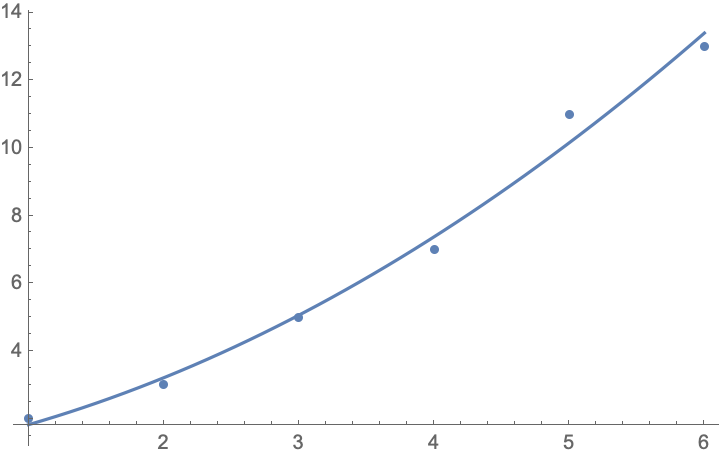
\includegraphics{physics--lagrangian-regression.png}


